\documentclass[a4paper,11pt]{exam}
\printanswers % pour imprimer les réponses (corrigé)
%\noprintanswers % Pour ne pas imprimer les réponses (énoncé)
\addpoints % Pour compter les points
% \noaddpoints % pour ne pas compter les points
%\qformat{\textbf{\thequestion ) } }
\qformat{\textbf{\thequestion )} \textit{(\thepoints)} \\  } % Pour définir le style des questions (facultatif)
\usepackage{color} % définit une nouvelle couleur
\shadedsolutions % définit le style des réponses
% \framedsolutions % définit le style des réponses
\definecolor{SolutionColor}{rgb}{0.8,0.9,1} % bleu ciel
\renewcommand{\solutiontitle}{\noindent\textbf{Solution:}\par\noindent} % Définit le titre des solutions




\makeatletter

\def\maketitle{{\centering%
	\par{\huge\textbf{\@title}}%
	\par{\@date}%
	\par}}

\makeatother

\lhead{NOM Pr\'enom :}
\rhead{\textbf{Les r\'eponses doivent \^etre justifi\'ees}}
\cfoot{\thepage / \pageref{LastPage}}


%\usepackage{../../pas-math}
%\usepackage{../../moncours}


%\usepackage{pas-cours}
%-------------------------------------------------------------------------------
%          -Packages nécessaires pour écrire en Français et en UTF8-
%-------------------------------------------------------------------------------
\usepackage[utf8]{inputenc}
\usepackage[frenchb]{babel}
\usepackage[T1]{fontenc}
\usepackage{lmodern}
\usepackage{textcomp}



%-------------------------------------------------------------------------------

%-------------------------------------------------------------------------------
%                          -Outils de mise en forme-
%-------------------------------------------------------------------------------
\usepackage{hyperref}
\hypersetup{pdfstartview=XYZ}
%\usepackage{enumerate}
\usepackage{graphicx}
\usepackage{multicol}
\usepackage{tabularx}
\usepackage{multirow}


\usepackage{anysize} %%pour pouvoir mettre les marges qu'on veut
%\marginsize{2.5cm}{2.5cm}{2.5cm}{2.5cm}

\usepackage{indentfirst} %%pour que les premier paragraphes soient aussi indentés
\usepackage{verbatim}
\usepackage{enumitem}
\usepackage[usenames,dvipsnames,svgnames,table]{xcolor}

\usepackage{variations}

%-------------------------------------------------------------------------------


%-------------------------------------------------------------------------------
%                  -Nécessaires pour écrire des mathématiques-
%-------------------------------------------------------------------------------
\usepackage{amsfonts}
\usepackage{amssymb}
\usepackage{amsmath}
\usepackage{amsthm}
\usepackage{tikz}
\usepackage{xlop}
%-------------------------------------------------------------------------------



%-------------------------------------------------------------------------------


%-------------------------------------------------------------------------------
%                    - Mise en forme avancée
%-------------------------------------------------------------------------------

\usepackage{ifthen}
\usepackage{ifmtarg}


\newcommand{\ifTrue}[2]{\ifthenelse{\equal{#1}{true}}{#2}{$\qquad \qquad$}}

%-------------------------------------------------------------------------------

%-------------------------------------------------------------------------------
%                     -Mise en forme d'exercices-
%-------------------------------------------------------------------------------
%\newtheoremstyle{exostyle}
%{\topsep}% espace avant
%{\topsep}% espace apres
%{}% Police utilisee par le style de thm
%{}% Indentation (vide = aucune, \parindent = indentation paragraphe)
%{\bfseries}% Police du titre de thm
%{.}% Signe de ponctuation apres le titre du thm
%{ }% Espace apres le titre du thm (\newline = linebreak)
%{\thmname{#1}\thmnumber{ #2}\thmnote{. \normalfont{\textit{#3}}}}% composants du titre du thm : \thmname = nom du thm, \thmnumber = numéro du thm, \thmnote = sous-titre du thm

%\theoremstyle{exostyle}
%\newtheorem{exercice}{Exercice}
%
%\newenvironment{questions}{
%\begin{enumerate}[\hspace{12pt}\bfseries\itshape a.]}{\end{enumerate}
%} %mettre un 1 à la place du a si on veut des numéros au lieu de lettres pour les questions 
%-------------------------------------------------------------------------------

%-------------------------------------------------------------------------------
%                    - Mise en forme de tableaux -
%-------------------------------------------------------------------------------

\renewcommand{\arraystretch}{1.7}

\setlength{\tabcolsep}{1.2cm}

%-------------------------------------------------------------------------------



%-------------------------------------------------------------------------------
%                    - Racourcis d'écriture -
%-------------------------------------------------------------------------------

% Angles orientés (couples de vecteurs)
\newcommand{\aopp}[2]{(\vec{#1}, \vec{#2})} %Les deuc vecteurs sont positifs
\newcommand{\aopn}[2]{(\vec{#1}, -\vec{#2})} %Le second vecteur est négatif
\newcommand{\aonp}[2]{(-\vec{#1}, \vec{#2})} %Le premier vecteur est négatif
\newcommand{\aonn}[2]{(-\vec{#1}, -\vec{#2})} %Les deux vecteurs sont négatifs

%Ensembles mathématiques
\newcommand{\naturels}{\mathbb{N}} %Nombres naturels
\newcommand{\relatifs}{\mathbb{Z}} %Nombres relatifs
\newcommand{\rationnels}{\mathbb{Q}} %Nombres rationnels
\newcommand{\reels}{\mathbb{R}} %Nombres réels
\newcommand{\complexes}{\mathbb{C}} %Nombres complexes


%Intégration des parenthèses aux cosinus
\newcommand{\cosP}[1]{\cos\left(#1\right)}
\newcommand{\sinP}[1]{\sin\left(#1\right)}


%Probas stats
\newcommand{\stat}{statistique}
\newcommand{\stats}{statistiques}
%-------------------------------------------------------------------------------

%-------------------------------------------------------------------------------
%                    - Mise en page -
%-------------------------------------------------------------------------------

\newcommand{\twoCol}[1]{\begin{multicols}{2}#1\end{multicols}}


\setenumerate[1]{font=\bfseries,label=\textit{\alph*})}
\setenumerate[2]{font=\bfseries,label=\arabic*)}


%-------------------------------------------------------------------------------
%                    - Elements cours -
%-------------------------------------------------------------------------------




\usepackage{tabu}

%\usepackage{fullpage}
\author{\ }
\date{$1^{er}$ Avril 2018}
\title{$T^{le}$ $ST_2S$ : DS num\'ero 4}


\begin{document}
%	\usepackage{fancyhdr}
%	
%	\pagestyle{fancy}
%	\fancyhf{}
	%\rhead{Share\LaTeX}

	\maketitle




\section{Un arbre pondéré est donné (7 points)}

\emph{Les résulats approchés sont à arrondir à $10^{-4}$.}

Pour combattre les risques d'épidémie dus à une maladie, un laboratoire à mis au point un vaccin. Il a testé ce vaccin et a obtenu les données suivantes :
\begin{itemize}
	\item la probabilité qu'un individu soit malade sachant qu'il a été vacciné est égale à \num{0.09};
	\item la probabilité qu'un individu soit malade sachant qu'il n'a pas été vacciné est égale à \num{0.5}.
\end{itemize} 

Un quart de la population a été vaccinée contre la maladie. Une épidémie survient. Pour une personne choisie au hasard dans la population, on notera $M$l'événement <<être malade>>, $\bar{M}$ l'événement contraire, $V$ l'événement <<être vaccine>>, $\bar{V}$ l'événement contraire.

\begin{questions}
	\question[2] Compléter l'arbre de probabilité traduisant les informations de l'énoncé :
	
	\begin{center}
		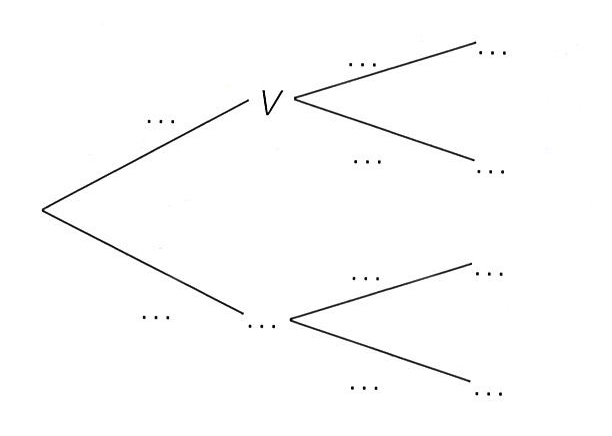
\includegraphics[scale=0.6]{arbre_pond}
	\end{center}

	\begin{solution}
		\begin{center}
			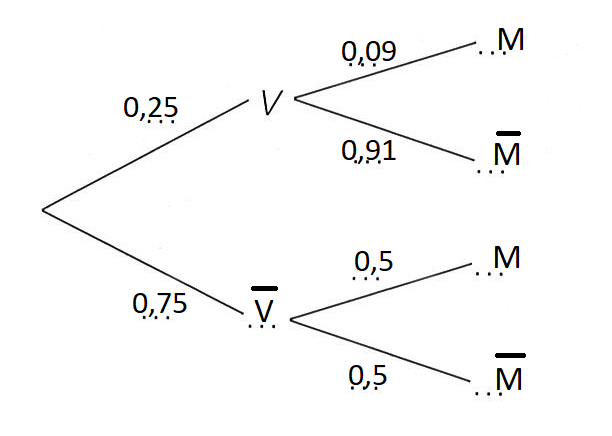
\includegraphics[scale=0.6]{arbre_pond2}
		\end{center}
	\end{solution}

	\question[1] Calculer la probabilité des événements $M \cap V$ et $M \cap \bar{V}$.
	\begin{solution}
		Calcul de $P(M \cap V)$ :
		
		\begin{eqnarray*}
			P(M \cap V) &=& P(V) \times P_V(M) \\
			P(M \cap V) &=& \num{0.25} \times \num{0.09} \\
			P(M \cap V) &=& \num{0.0225}
		\end{eqnarray*}
	
		Calcul de $P(M \cap \bar{V})$ :
		
		\begin{eqnarray*}
			P(M \cap \bar{V}) &=& P(\bar{V}) \times P_{\bar{V}}(M) \\
			P(M \cap \bar{V}) &=& \num{0.75} \times \num{0.5} \\
			P(M \cap \bar{V}) &=& \num{0.375}
		\end{eqnarray*}
	
	La probabilité de l'événement $M \cap V$ est \num{0.0225} et celle de $M \cap \bar{V}$ est \num{0.375}.
	\end{solution}
	
	\question[2] Calculer la probabilité de l'événement $M$ puis de l'événement $\bar{M}$.
	\begin{solution}
		Calcul de $P(M) $ :
		
		\begin{eqnarray*}
			P(M) &=& P(M \cap V) + P(M \cap \bar{V}) \\
			P(M) &=& \num{0.0225} + \num{0.375} \\
			P(M) &=& \num{0.3975}
		\end{eqnarray*}
	
		Calcul de $P(\bar{M}) $ :
		
		\begin{eqnarray*}
			P(\bar{M}) &=& 1 - P(M) \\
			P(\bar{M}) &=& 1 -  \num{0.3975} \\
			P(\bar{M}) &=& \num{0.6025}
		\end{eqnarray*}
	
		La probabilité de l'événement $M$ est \num{0.3975} et celle de $\bar{M}$ est \num{0.6025}.
	\end{solution}
	
	\question[2] Sachant qu'un individu choisi au hasard dans la population n'est pas malade, quelle est la probabilité qu'il ait été vacciné ?
	\begin{solution}
		Calcul de la probabilité qu'un individu soit vacciné sachant qu'il n'est pas malade :
		\begin{eqnarray*}
			P_{\bar{M}}(V) &=& \dfrac{P(V \cap \bar{M})}{P(\bar{M})}\\
			P_{\bar{M}}(V) &=& \dfrac{P(V) \times P_V(\bar{M})}{P(\bar{M})}\\
			P_{\bar{M}}(V) &=& \dfrac{\num{0.25} \times \num{0.91}}{\num{0.6025}}\\
			P_{\bar{M}}(V) &\approx& \num{0.3776}
		\end{eqnarray*}
	
	La probabilité qu'un individu non malade ait été vacciné est \num{0.3776}.
	\end{solution}
\end{questions}  
%\section{Un QCM (6 points)}

\textit{Cet exercice se présente sous la forme d'un questionnaire à choix multiple (QCM). Pour chaque question, trois réponses sont proposées. Une seule réponses est correcte. On demande de choisir celle que vous pensez être correcte.
}


On donne le tableau de variation d'une fonction $f$ définie et dérivable sur l'intervalle $[-12, 20]$ :

\begin{center}

	\begin{tikzpicture}[scale=0.8]
		\tkzTabInit{$x$/1.5,$f'(x)$/1.5,$f(x)$/4}{$-12$, $-5$, $7$, $20$}
		\tkzTabLine { ,- ,z , +, z, -}
		\tkzTabVar{+/$7$,-/$-4$,+/$-1$,-/$-6$}
	\end{tikzpicture}

\end{center}

\begin{questions}
	\question[1] On peut dire que :
	
		\begin{checkboxes}
			\choice $f$ est positive sur l'intervalle $[-12; -5]$.
			\choice $f$ est positive sur l'intervalle $[7; 20]$.
			\correctchoice $f$ est négative sur l'intervalle $[-5; 20]$.
		\end{checkboxes}
	
		
	\question[1] L'équation $f(x)=2$ possède 
	
	\begin{oneparcheckboxes}
		
		\correctchoice une seule solution ;
		\choice aucune solution ; 
		\choice on ne peut pas répondre.
	\end{oneparcheckboxes}	

	\question[1] On cherche à comparer $f'(0)$ et $f'(8)$ :

\begin{oneparcheckboxes}
	
	
	\choice $f'(0) < f'(8)$
	\correctchoice $f'(0) > f'(8)$
	\choice on ne peut pas répondre.
\end{oneparcheckboxes}

	\question[1] On cherche à comparer $f(0)$ et $f(8)$ :
	
	\begin{oneparcheckboxes}
		
		
		\choice $f(0) < f(8)$
		\choice $f(0) > f(8)$
		\correctchoice on ne peut pas répondre.
	\end{oneparcheckboxes}



	\question[1] Une équation de la tangente à la courbe représentative de la fonction $f$ au point d'abscisse 20 est :
	
	\begin{oneparcheckboxes}
		
		
		\choice $y = 20x - 6$
		\choice $y = -x - 6$
		\correctchoice $y = -x + 14$
	\end{oneparcheckboxes}

	\question[1] On désigne par $\mathcal{C}$ la courbe représentative de $f$ dans un repère orthogonal.
	
	\begin{oneparcheckboxes}
		
		\choice Il n'existe aucun point où la tangente à la courbe $\mathcal{C}$ est parallèle à l'axe des abscisses.
		\choice Il existe un seul point où la tangente à la courbe $\mathcal{C}$ est parallèle à l'axe des abscisses.
		\correctchoice Il existe deux points où la tangente à la courbe $\mathcal{C}$ est parallèle à l'axe des abscisses.
	\end{oneparcheckboxes}	
\end{questions}

\newpage 
\section{Un jeu de cartes (5 points)}

On tire au hasard une carte dans un jeu de trente-deux. Les trente-deux événements élémentaires sont équiprobables.

\begin{questions}
	
	
	\question[1] Donner deux événements incompatibles.
	\begin{solution}
		Les événements <<la carte tirée est un c\oe ur>> et <<la carte tirée est un pique>> sont incompatibles.
	\end{solution}
	
	\question Les événements $A$ et $B$ sont-ils indépendants ?
	
		\begin{parts}
			\part[2] $A$ : <<la carte tirée est une dame >>; $B$ : <<la carte tirée est noire>>.
			
			\begin{solution}
				\begin{eqnarray}
					P(A) &=& \dfrac{4}{32} = \dfrac{1}{8} \\
					P(B) &=& \dfrac{1}{2}\\
					P(A \cap B) &= & \dfrac{2}{32} = \dfrac{1}{16}\\
					P(A) \times P(B) &=& \dfrac{1 \times 1}{8 \times 2} = \dfrac{1}{16}
				\end{eqnarray}
				
				On a $P(A\cap B)  = P(A) \times P(B)$, donc les événements $A$ et $B$ sont indépendants.
			\end{solution}
			
			\part[2] $A$ : <<la carte tirée est une dame >>; $B$ : <<la carte tirée est une figure>>.
			
			\begin{solution}
				\begin{eqnarray}
				P(A) &=& \dfrac{4}{32} = \dfrac{1}{8} \\
				P(B) &=& \dfrac{12}{32} = \dfrac{3}{8}\\
				P(A \cap B) &= & \dfrac{4}{32} = \dfrac{1}{8}\\
				P(A) \times P(B) &=& \dfrac{1 \times 3}{8 \times 8} = \dfrac{3}{64}
				\end{eqnarray}
				
				On a $P(A\cap B)  \neq P(A) \times P(B)$, donc les événements $A$ et $B$ ne sont pas indépendants.
			\end{solution}
		\end{parts}
\end{questions} 



\newpage 
\section{Tabac pendant la grossesse (8 points)}

En 2007, une enquête réalisé sur le lien de cause à effet entre l'état tabagique de la mère pendant la grossesse  et les troubles respiratoires de l'enfant. Cette enquête est réalisée sur un échantillon de 1500 enfants de 10 ans.
Chaque enfant est classé dans un des trois groupe suivants :
\begin{itemize}
	\item les asthmatiques;
	\item ceux qui présentent des troubles asthmatiformes (considérés comme non asthmatiques);
	\item ceux sans troubles.

\end{itemize}

Le recueil des données est réalisé sous couvert de l'anonymat auprès des professionnels médicaux, 1500 fiches de renseignements anonymes ont été créées.
Ces fiches indiquent que :

\begin{itemize}
	\item 1223 enfants n'ont aucun troubles.
	\item \num{4.8} \% des enfants sont asthmatiques ; 75 \% d'entre eux ont une mère ayant fumé pendant la grossesse.
	\item 16 \% des mères ont fumé pendant la grossesse.
	\item 40 \% des enfants ayant des allergies asthmatiformes ont une mère n'ayant pas fumé pendant la grossesse.
\end{itemize}

\begin{questions}
	\question[2] Compléter le tableau suivant :
	
	\begin{center}
		\begin{tabular}{|@{\ }l@{\ }|@{\ }c@{\ }|@{\ }c@{\ }|@{\ \ \ \ \ }c@{\ \ \ \ \ }|}
	\hline
                     & Mère fumeuse & Mère non fumeuse &  \\
                     & pendant la                       & pendant la                           & Total                \\
                     & grossesse                        & grossesse                            &                      \\
	\hline
	& & &\\
Enfants asthmatiques &                                  &                                      & 72                   \\
	& & &\\
	\hline
Enfants présentant   &                                  &                                      &                      \\
un trouble           & 123                              &                                      &                      \\
asthmatiforme        &                                  &                                      &                      \\
	\hline
Enfant ne            &                                  &                                      &                      \\
présentant           &                                  &                                      & 1223                 \\
aucun trouble        &                                  &                                      &                      \\
	\hline
Total                & 240                              &                                      & 1500                \\
	\hline
\end{tabular}
	\end{center}

	\begin{solution}
		\begin{center}
			\begin{tabular}{|@{\ }l@{\ }|@{\ }c@{\ }|@{\ }c@{\ }|@{\ \ \ \ \ }c@{\ \ \ \ \ }|}
	\hline
                     & Mère fumeuse & Mère non fumeuse &  \\
                     & pendant la                       & pendant la                           & Total                \\
                     & grossesse                        & grossesse                            &                      \\
	\hline
	& & &\\
Enfants asthmatiques &        54                        &    18                                & 72                   \\
	& & &\\
	\hline
Enfants présentant   &                                  &                                      &                      \\
un trouble           & 123                              &   226                                &  349                 \\
asthmatiforme        &                                  &                                      &                      \\
	\hline
Enfant ne            &                                  &                                      &                      \\
présentant           &   63                             &    1160                              & 1223                 \\
aucun trouble        &                                  &                                      &                      \\
	\hline
Total                & 240                              &      1260                            & 1500                \\
	\hline
\end{tabular}
		\end{center}
	\end{solution}

	\question On prélève au hasard une fiche de renseignement d'un enfant. ON admet que chacun des choix est équiprobable. On considère les événements suivants :
	
	\begin{itemize}
		\item $A$ : << La fiche indique que l'élève est asthmatique>>; 
		\item $T$ : << La fiche indique que l'élève présente des troubles asthmatiformes>>;
		\item $F$ : << La fiche indique que la mère a fumé pendant la grossesse>>;
	\end{itemize}

	Les résultats approchés sont à arrondir au millième.
	
	\begin{parts}
		\part[1\half] Calculer la probabilité des événements $T$ et $F$.
		
		\begin{solution}
			\begin{eqnarray*}
				P(T) &=& \frac{205}{1500} \approx \num{0.137} \\
				P(F) &=& \frac{240}{1500} = \num{0.16} \\
			\end{eqnarray*}
		\end{solution}
	
		\part[1\half] Définir par une phrase l'événement $T \cap F$ puis calculer sa probabilité.
		\begin{solution}
			L'événement $T \cap F$ est <<La fiche indique que l'élève présente des troubles asthmatiformes et sa mère a fumé pendant la grossesse. Sa probabilité est \num{0.082} ($\frac{123}{1500}$).
			 
		\end{solution}
		
		\part[1] Calculer la probabilité que l'enfant ait des troubles asthmatiformes ou que sa mère soit fumeuse.
		\begin{solution}
			\begin{eqnarray*}
				P(T \cup F) &=& P(T) + P(F) - P(T \cap F) \\
				P(T \cup F) &=& \num{0.137} + \num{0.16} - \num{0.082} \\
				P(T \cup F) &=& \num{0.215}
			\end{eqnarray*}
		
			La probabilité que l'enfant ait des troubles asthmatiques ou que sa mère soit fumeuse est \num{0.311}.
		\end{solution}
		
		\part[1] Calculer la probabilité que l'enfant soit asthmatique sachant que sa mère est fumeuse.
		\begin{solution}
			\begin{eqnarray*}
				P_F(A) &=& \frac{54}{240} \\
				P_F(A) &=& \num{0.225}\\
			\end{eqnarray*}
		
		La probabilité que l'enfant soit asthmatique sachant que sa mère est fumeuse est \num{0.225}.
		\end{solution}
	\end{parts}

	\question[1] On prélève au hasard une fiche parmi celles indiquant que la mère a fumé pendant la grossesse. Calculer la probabilité que l'enfant n'ait aucun trouble. 
	
	\begin{solution}
		Soit $N$ l'événement : <<La fiche tirée indique que l'élève ne présente aucun trouble>>.
		
		\begin{eqnarray*}
			P_F(N) &=& \frac{63}{240} \\
			P_F(N) &\approx&  \num{0.263}\\
		\end{eqnarray*}
	
	La probabilité que l'enfant n'ait aucun trouble sachant que sa mère a fumé pendant la grossesse est \num{0.263}.
	\end{solution}
\end{questions}




%\section{Effectifs étudiants}
	
	\begin{questions}
		\question En 2005, \num{125634} étudiants se sont inscrits en IUT. Environ \num{33.8}\% venaient de série technologiques. Combien d'élèves inscrits en IUT en 2005 venaient de séries technologiques ?
		\begin{solution}
			$ \num{125634} \times \dfrac{\num{33.8}}{100} = \num{42464.292} $ \\
			Soit environ \num{42465} étudiants issus de séries technologiques.
		\end{solution}
		
		\question Au lycée Marcel PAGNOL, 62 élèves sont inscrits en section ST2S, ce qui représente 8\% du total des élèves. Combien y a t-il d'élèves dans ce lycée ?
		\begin{solution}
			$ \dfrac{\num{62}}{\num{0.08}} = 775 $ \\
			Soit environ 775 élèves dans le lycée.
		\end{solution}
	\end{questions}

\label{LastPage}
	

\end{document}